%%%%%%%%%%%%%%%%%%%%%%%%%%%%%%%%%%%%%%%%%%%%%%%%%%%%%%%%%%%%%%%%%%%%%%%%%%%%%%%%
%2345678901234567890123456789012345678901234567890123456789012345678901234567890
%        1         2         3         4         5         6         7         8
\documentclass[letterpaper, 10 pt, conference]{ieeeconf}  % Comment this line out
                                                          % if you need a4paper
%\documentclass[a4paper, 10pt, conference]{ieeeconf}      % Use this line for a4

\usepackage{float}
                                                          % paper
% uso paquete bookmark para tener bien los outlines.
\usepackage{bookmark}

% Configuro el idioma.
\usepackage[utf8]{inputenc} % Importante para mantener acentos.
\usepackage[spanish, activeacute]{babel} % Requiere: texlive-lang-spanish. Por primera vez hay que ejecutar: texconfig init> log

% Paquete para poder usar acentos en $$.
\usepackage{mathtools}
%\setmathfont{XITS math}

% Para los diagramas de flujo
\usepackage{tikz}
\usetikzlibrary{shapes.geometric, arrows}

% Elementos del diagrama
\tikzstyle{startstop} = [rectangle, rounded corners, 
minimum width=6em, 
minimum height=2em,
text centered, 
draw=black, 
fill=red!30]

\tikzstyle{io} = [trapezium, 
trapezium stretches=true, % A later addition
trapezium left angle=70, 
trapezium right angle=110, 
minimum width=6em, 
minimum height=2em, text centered, 
draw=black, fill=blue!30]

\tikzstyle{block} = [rectangle, 
minimum width=8em, 
minimum height=3em, 
text centered, 
text width=7.5em, 
draw=black, 
fill=white!30]

\tikzstyle{def} = [rectangle, 
minimum width=14em, 
minimum height=3em, 
text centered, 
text width=12em, 
draw=black, 
fill=purple!30]

\tikzstyle{swap_proccess} = [rectangle, 
minimum width=8em, 
minimum height=2em, 
text centered, 
text width=8em, 
draw=black, 
fill=orange!30]

\tikzstyle{process} = [rectangle, 
minimum width=6em, 
minimum height=2em, 
text centered, 
text width=6em, 
draw=black, 
fill=orange!30]

\tikzstyle{decision} = [diamond, 
minimum width=6em, 
minimum height=6em, 
text centered, 
draw=black, 
fill=green!30]
\tikzstyle{arrow} = [thick,->,>=stealth]

\usepackage{siunitx}

% package to get \url
\usepackage{hyperref}
\hypersetup{
  colorlinks=true,
  linkcolor=magenta,
  filecolor=magenta,
  citecolor=magenta,      
  urlcolor=magenta,
}

% Graficos electrónicos
\usepackage[RPvoltages]{circuitikz}

\IEEEoverridecommandlockouts                              % This command is only
                                                          % needed if you want to
                                                          % use the \thanks command
\overrideIEEEmargins
% See the \addtolength command later in the file to balance the column lengths
% on the last page of the document

\usepackage{graphicx}
\usepackage{graphics}

% styling for matlab/octave code.
\usepackage{matlab-prettifier}
% Configuracion, con esto puede agregar ñ.
\lstset{
  literate={ñ}{{\~n}}1
}

\usepackage{listings}

% The following packages can be found on http:\\www.ctan.org
%\usepackage{graphics} % for pdf, bitmapped graphics files
%\usepackage{epsfig} % for postscript graphics files
%\usepackage{mathptmx} % assumes new font selection scheme installed
%\usepackage{times} % assumes new font selection scheme installed
\usepackage{amsmath} % assumes amsmath package installed
%\usepackage{amssymb}  % assumes amsmath package installed

\title{\LARGE \bf Trabajo Práctico N° 1 Ejercicio 3}

\author{
  Tom\'as Vidal\\
  {\it Control de sistemas biológicos}\\
  {\it Facultad de Ingenier\'ia, UNLP, La Plata, Argentina.}\\
  {\it 17 de Septiembre, 2024.}
}                                            % <-this % stops a space
% comienzo
% INTRO

% Figura
\newcommand{\image}[2] {
  \begin{figure}[H]
    \centering
    \includegraphics[width=0.43\textwidth]{./#1.png}
    \caption{#2}
    \label{fig:#1}
  \end{figure}
}

% Codigo
% \begin{lstlisting}[style=Matlab-editor]
% % el código va aca
% dispc("HELLO WORLD");
% \end{lstlisting}

\begin{document}
% - - - - - - - - - - - - - - - - - - - - - - - - - - - - - -  TITLE
\begin{titlepage}
	\centering
	\null\vspace{4cm} % Adjust this value to push everything down
	{\LARGE \textbf{Trabajo Práctico N° 1 Ejercicio 3} \par}
	\vspace{2cm}
	{\large Tomás Vidal \par}
	{\itshape Control de sistemas biológicos \par}
	{\itshape Facultad de Ingeniería, UNLP, La Plata, Argentina. \par}
	{\itshape 17 de Septiembre, 2024. \par}
	\vspace{2cm}
	
\includegraphics[width=0.55\textwidth]{unlp_logo.png}
	\vfill % Pushes the content to properly center vertically
\end{titlepage}
% - - - - - - - - - - - - - - - - - - - - - - - - - - - - - -

\section{Introducción}
A continuación se muestran los resultados de simular la \textbf{producción} de \textit{polihidroxibutirato} (PHB)\footnote{El polihidroxibutirato (PHB) es un biopolímero perteneciente a la familia de los poliésteres, producido por diversas bacterias como reserva de carbono y energía. Es biodegradable y biocompatible, lo que lo hace una alternativa ecológica a los plásticos convencionales en aplicaciones médicas y envasado sostenible.}, y el \textbf{crecimiento} de la bacteria que lo produce para 3 casos diferentes alimentaciones de sustrato: \textbf{sin alimentación}, \textbf{alimentación constante} y \textbf{alimentación exponencial}. \\
Las etapas de producción y crecimiento difieren en que la última requiere de nitrógeno, en cambio la etapa de producción de plástico require ausencia del mismo.

\section{Modelo}
El modelo a simular es el siguiente:

\begin{equation*}
	\begin{cases}
    k_{S1} S + k_N N \xrightarrow{r_x} X + k_{P1} P \\
    k_{S2} S \xrightarrow{r_p} P
	\end{cases}
\end{equation*}

Que se puede llevar al siguiente sistema de ecuaciones:

\begin{equation*}
	\begin{cases}
    \dot{x} = r_{x} \\
    \dot{s} = -K_{s1}r_{x}  + D_{s}(s_{in}  - s) \\
    \dot{s} = -K_{s2}r_{p}  + D_{s}(s_{in}  - s) \\
    \dot{n} = -K_{N}r_{x}  + D_{n}(n_{in}  - n) \\
    \dot{p} = K_{p1}r_{p} \\
	\end{cases}
\end{equation*}

Y representándolo en su forma vectorial se tiene:

\vspace{0.35cm}

$
\begin{bmatrix} \dot{x} \\ \dot{s} \\ \dot{n} \\ \dot{p} \end{bmatrix}
=
\begin{bmatrix} 1 & 0 \\ -K_{s1} & -K_{s2} \\ -K_{N} & 0 \\ K_{P1} & 1 \end{bmatrix}
.
\begin{bmatrix} r_{x} \\ r_{p} \end{bmatrix}
+
\begin{pmatrix}
  \begin{bmatrix} 0 & 0 \\ S_{in} & 0 \\ 0 & n_{in} \\ 0 & 0 \end{bmatrix}
  -
  \begin{bmatrix} x \\ s \\ n \\ p \end{bmatrix}
  .
  \begin{bmatrix} 1 & 1 \end{bmatrix}
\end{pmatrix}
.
  \begin{bmatrix} D_{s} \\ D_{n} \end{bmatrix}
$

\vspace{1cm}

Los modelos cinéticos empleados son:

\begin{equation*}
\mu(s,n) = \mu_{\text{max}} \frac{s}{K_S + s + \frac{s^2}{K_{is}}} \cdot \frac{n}{K_n + n}
\end{equation*}

\begin{equation*}
q_p(s,n) = q_{p\text{max}} \frac{s}{K_{ps} + s + \frac{s^2}{K_{ips}}} \cdot \frac{K_{ipn}}{K_{ipn} + n}
\end{equation*}

Para realizar la simulación se hizo uso de simulink, a continuación se muestran los dos casos para cuando no se alimenta o se alimenta constantemente con sustrato, y el caso para cuando se alimenta exponencialmente con sustrato.

\begin{figure}[H]
  \centering
  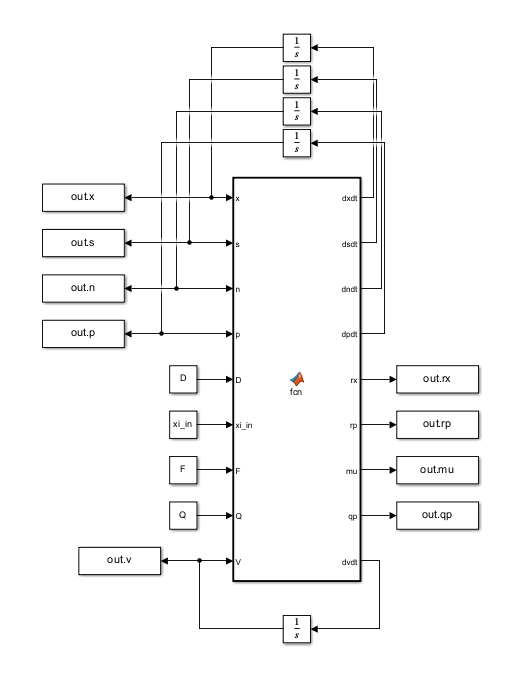
\includegraphics[width=0.43\textwidth]{./Images_tp1/simulink1.png}
  \caption{Simulación para el caso de alimentación constante}
  \label{fig:simulink1}
\end{figure}
\begin{figure}[H]
  \centering
  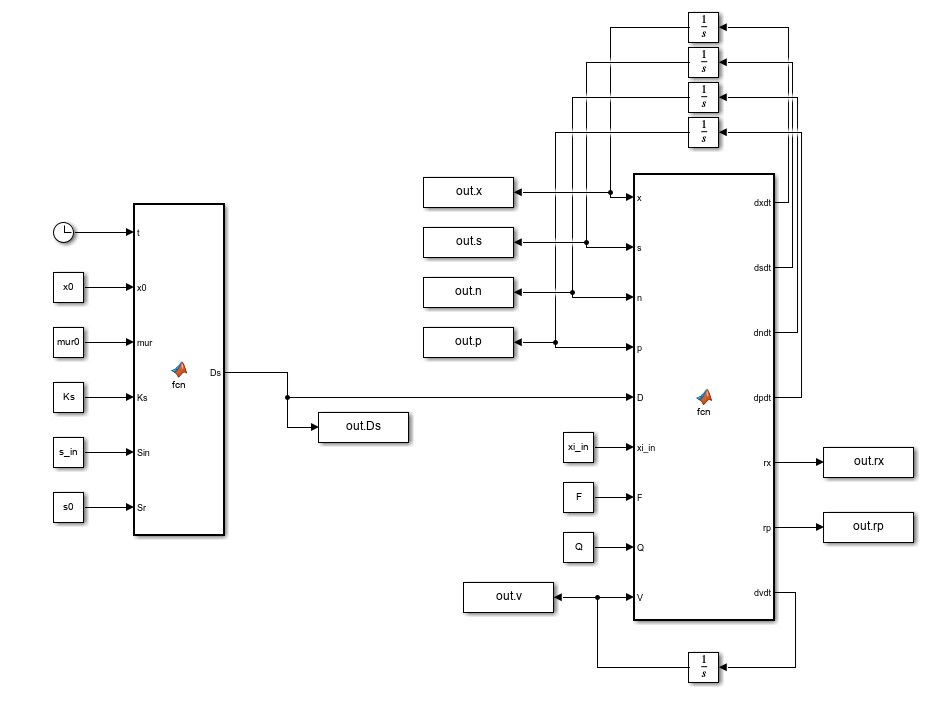
\includegraphics[width=0.43\textwidth]{./Images_tp1/simulink2.png}
  \caption{Simulación para el caso de alimentación exponencial}
  \label{fig:simulink2}
\end{figure}

\section{Sin alimentación de sustrato}

A continuación se muestran las simulaciones del caso donde no hay alimentación de sustrato, es decir $D_{s}=D_{n}=0$, que es el caso donde se hace un \textbf{batch}, se comienzan las etapas con ciertos valores de sustrato y nitrógeno, y se deja que el sistema evolucione sin cambiar la masa neta.

\subsection{Etapa de crecimiento}

\begin{figure}[H]
  \centering
  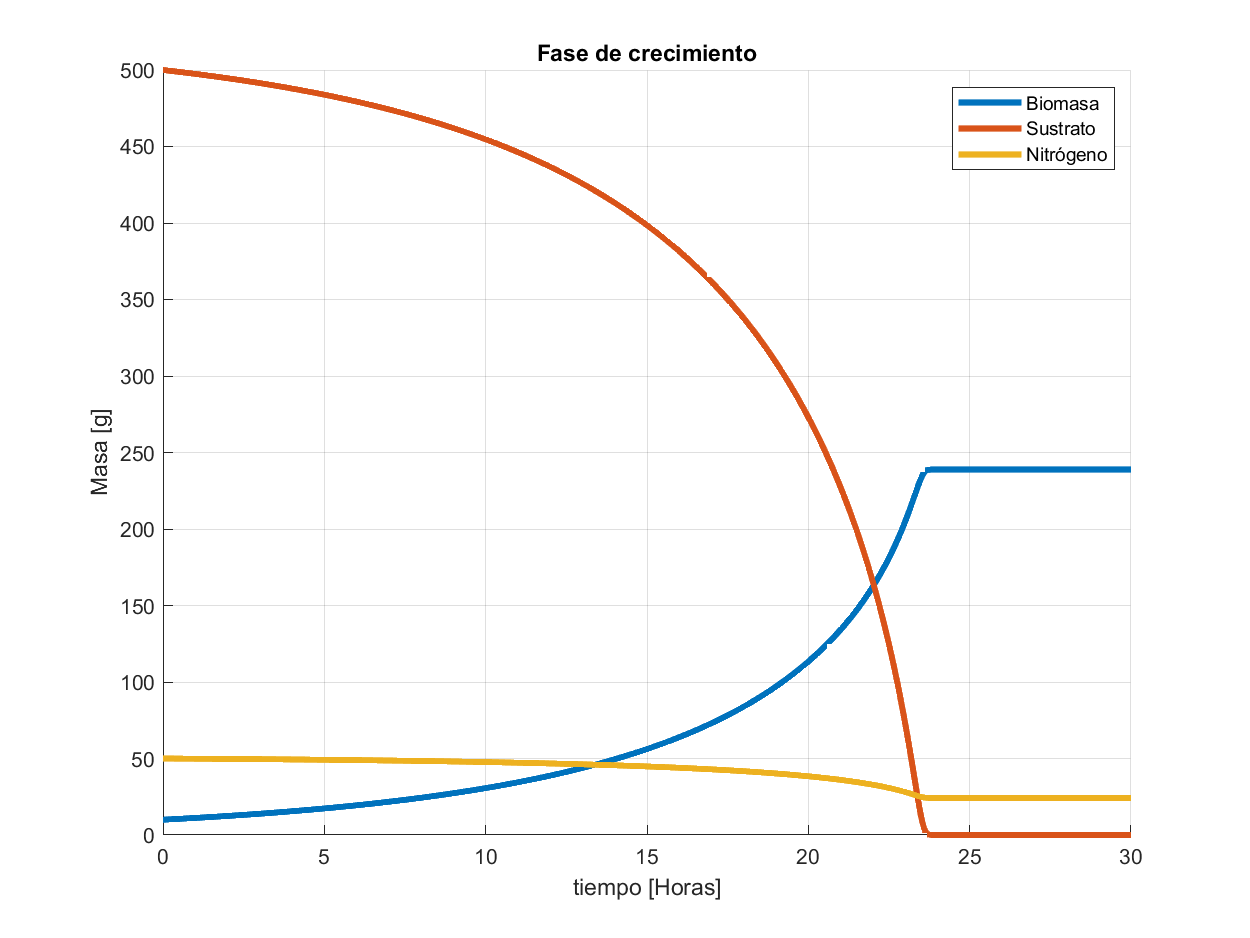
\includegraphics[width=0.43\textwidth]{./Images_tp1/D0_crecimiento_completo.png}
  \caption{Etapa de crecimiento sin alimentación de sustrato}
  \label{fig:D0_whole}
\end{figure}

\begin{figure}[H]
  \centering
  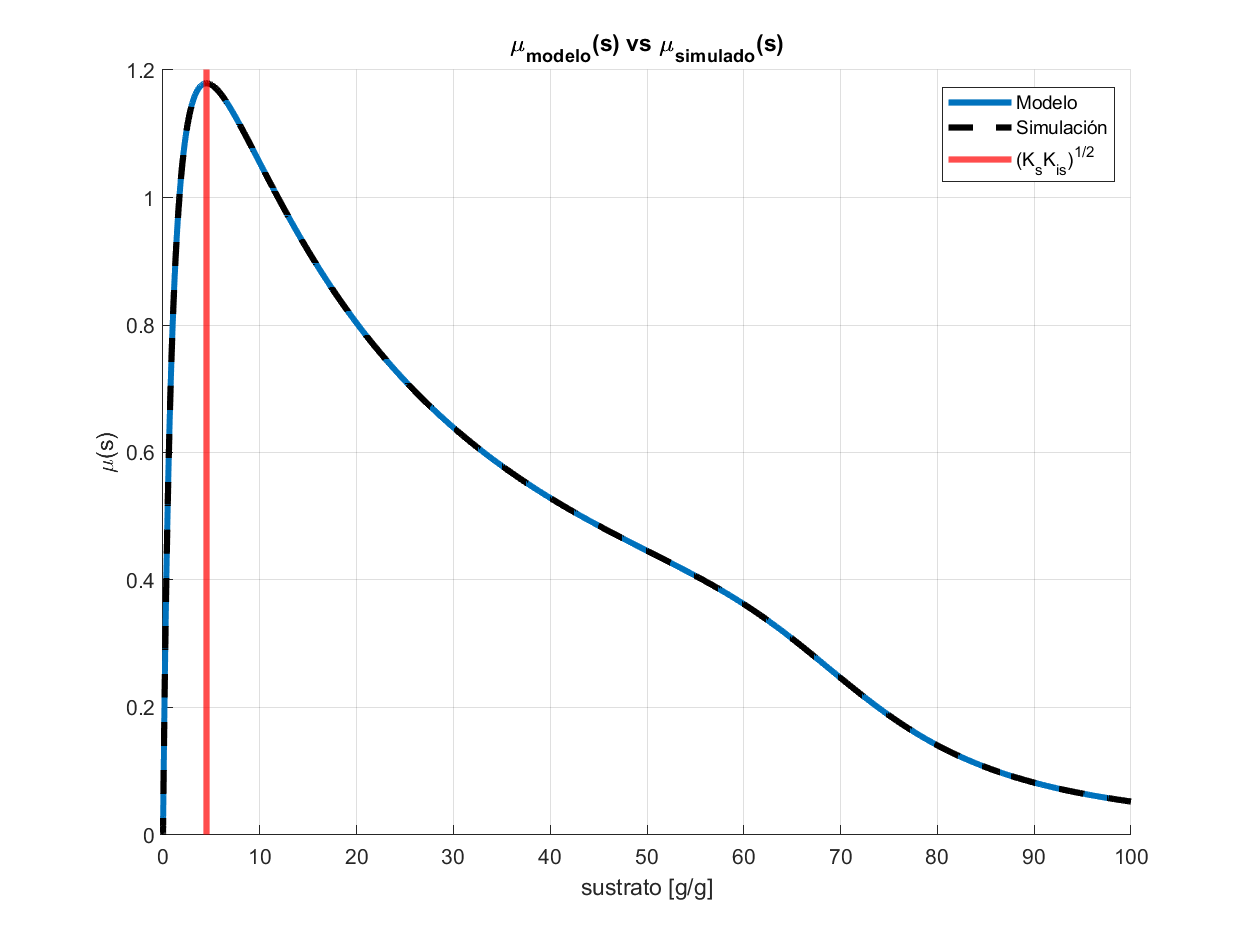
\includegraphics[width=0.43\textwidth]{./Images_tp1/D0_mus.png}
  \caption{Modelo cinético $\mu(s)$ en etapa de crecimiento}
  \label{fig:D0_mu}
\end{figure}

\begin{figure}[H]
  \centering
  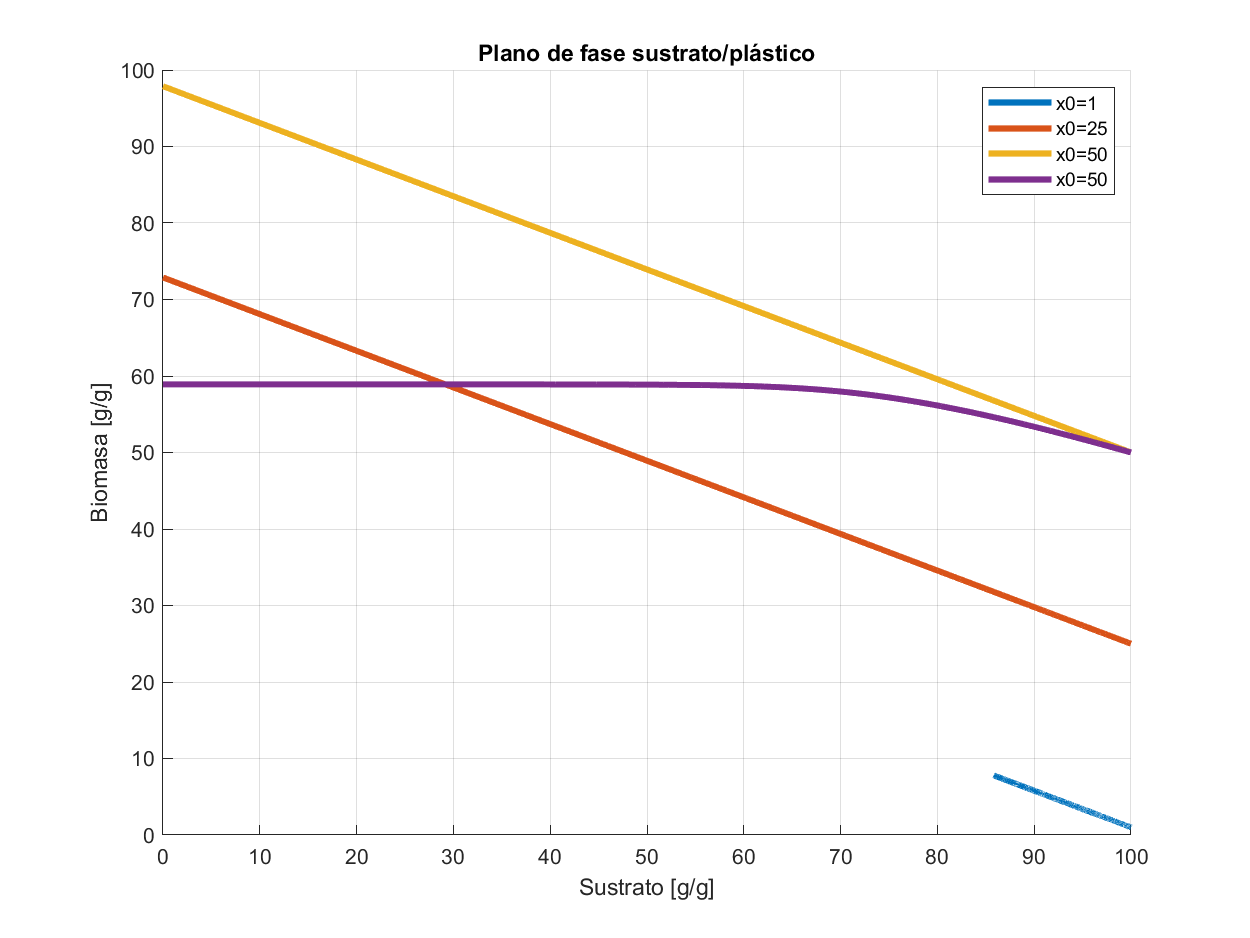
\includegraphics[width=0.43\textwidth]{./Images_tp1/D0_plano_fase.png}
  \caption{Plano de fase Sustrato/Biomasa en la etapa de crecimiento}
  \label{fig:D0_fase}
\end{figure}

Como era de esperar se tiene un crecimiento exponencial de biomasa y, un decrecimiento exponencial de sustrato. Además se tiene que los modelos cinéticos son correctos durante la simulación, se llega al máximo en \textit{aproximadamente} $\sqrt{K_{s}K_{is}}$. También se tiene la recta esperada en el plano de fase.

\subsection{Fase de producción de plástico}

\begin{figure}[H]
  \centering
  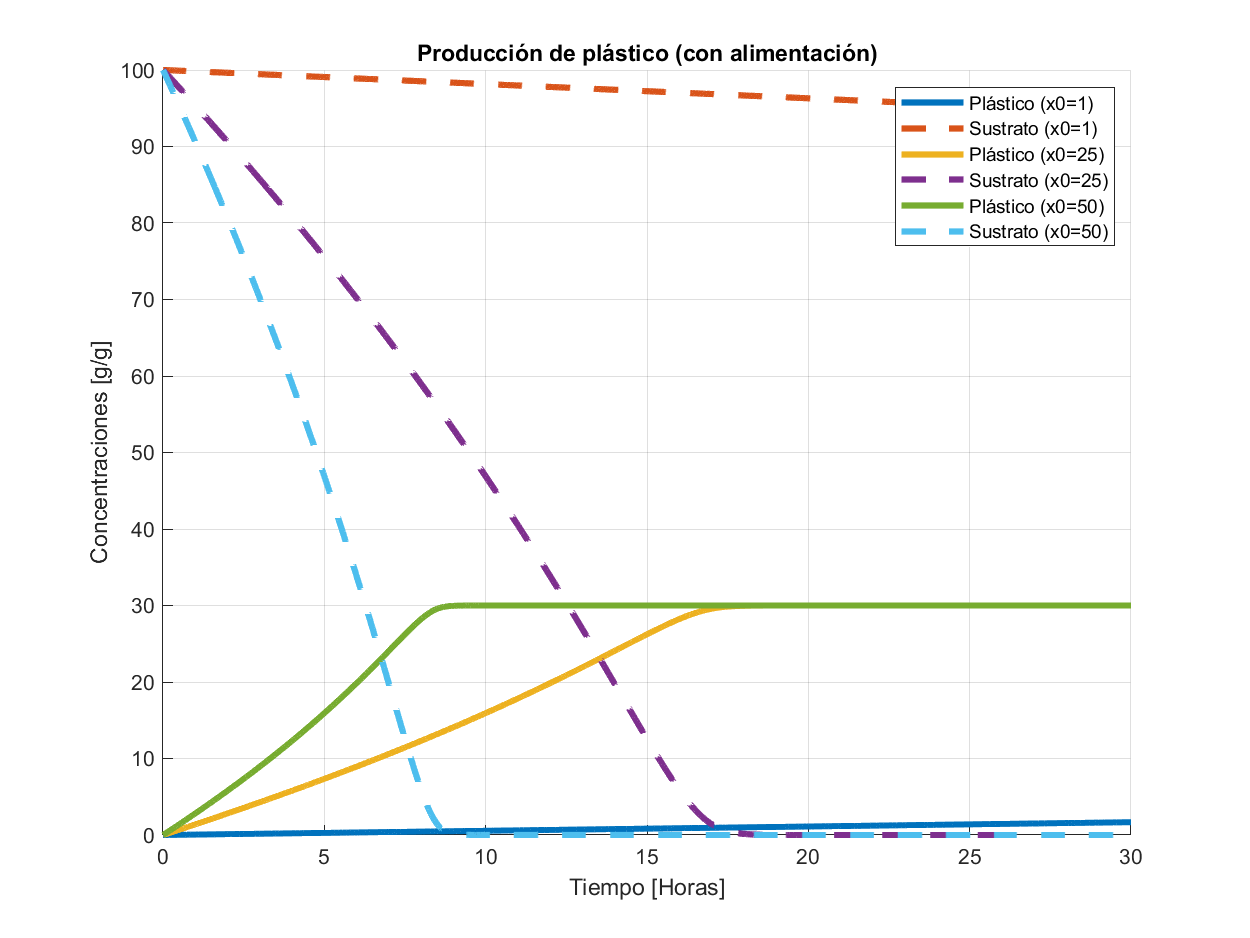
\includegraphics[width=0.43\textwidth]{./Images_tp1/D0_prod_completa.png}
  \caption{Etapa de producción de plástico con ``suficiente'' biomasa}
  \label{fig:D0_prod_completa}
\end{figure}

\begin{figure}[H]
  \centering
  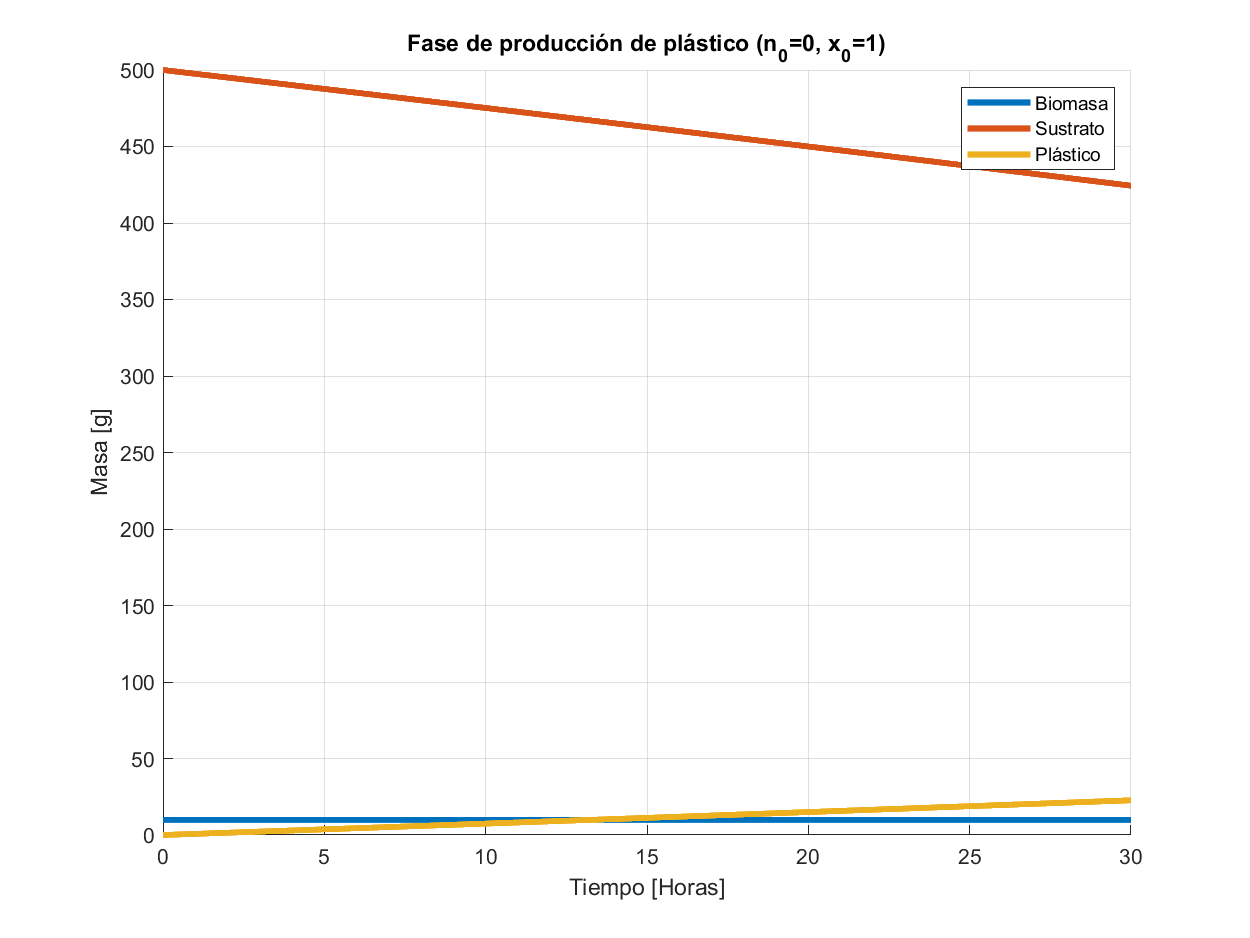
\includegraphics[width=0.43\textwidth]{./Images_tp1/D0_prod_completa_min_biomass.png}
  \caption{Etapa de producción de plástico con ``poca'' biomasa}
  \label{fig:D0_prod_completa_min_biomass}
\end{figure}

\begin{figure}[H]
  \centering
  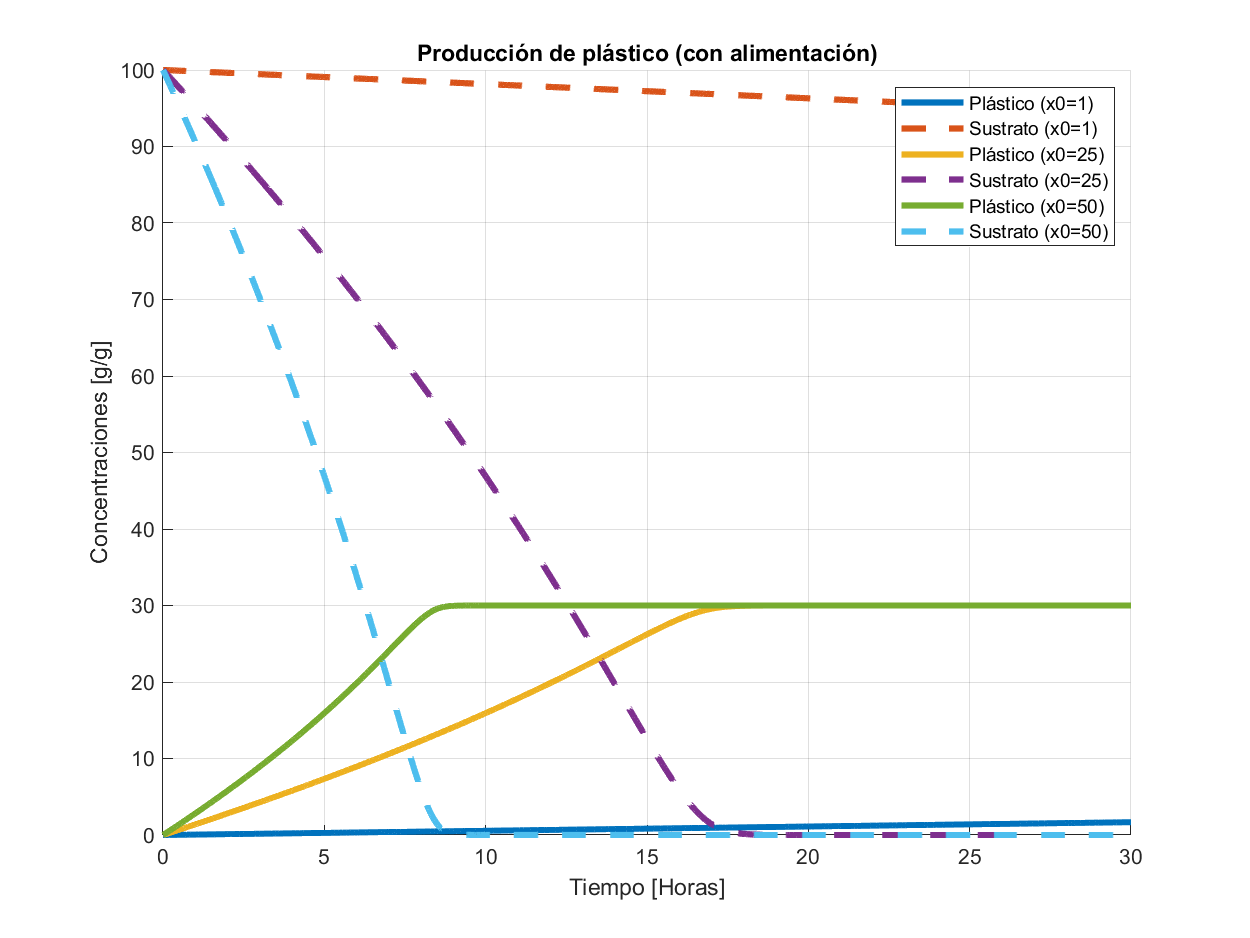
\includegraphics[width=0.43\textwidth]{./Images_tp1/D0_plano_fase_plastic.png}
  \caption{Plano de fase Sustrato/Plástico en la etapa de producción}
  \label{fig:D0_fase_plastic}
\end{figure}

En la figura \ref{fig:D0_prod_completa} se puede observar que después de 10 horas, con 200 gramos de biomasa, \textbf{se obtuvieron 150 gramos de plástico}, a partir de los 500 gramos de sustrato que se consumieron. También se simulo un caso donde la biomasa es poca, en comparación a la cantidad de sustrato y los tiempos de producción, y no se alcanza a consumir el sustrato en las 30 horas de simulación.

\section{Con alimentación de sustrato constante}

\subsection{Fase de crecimiento}

En esta fase se simula cuando se alimenta constantemente para diferentes valores de dilución

\begin{figure}[H]
  \centering
  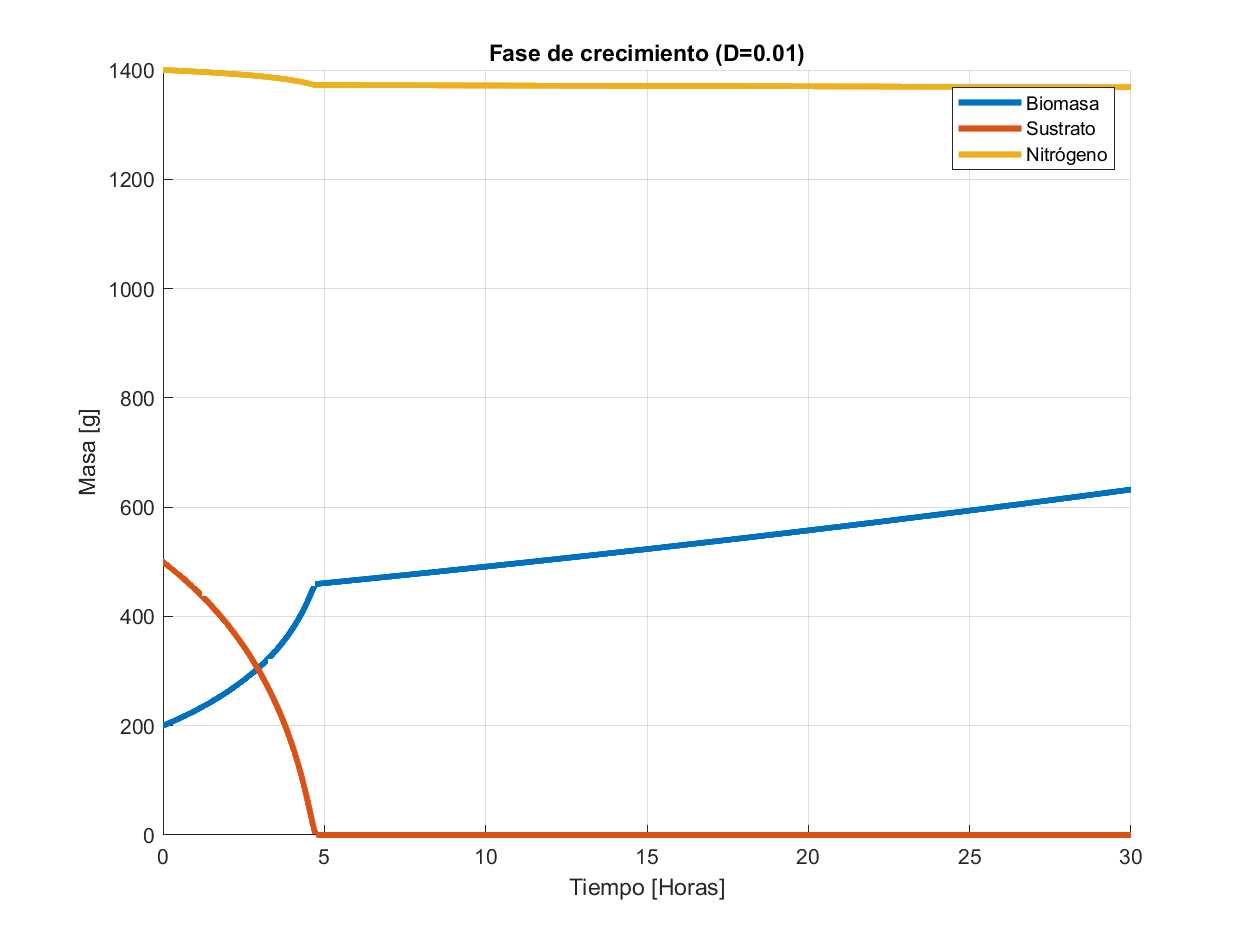
\includegraphics[width=0.43\textwidth]{./Images_tp1/D1_growth_complete_1.png}
  \caption{Fase de crecimiento con alimentación constante}
\end{figure}
\begin{figure}[H]
  \centering
  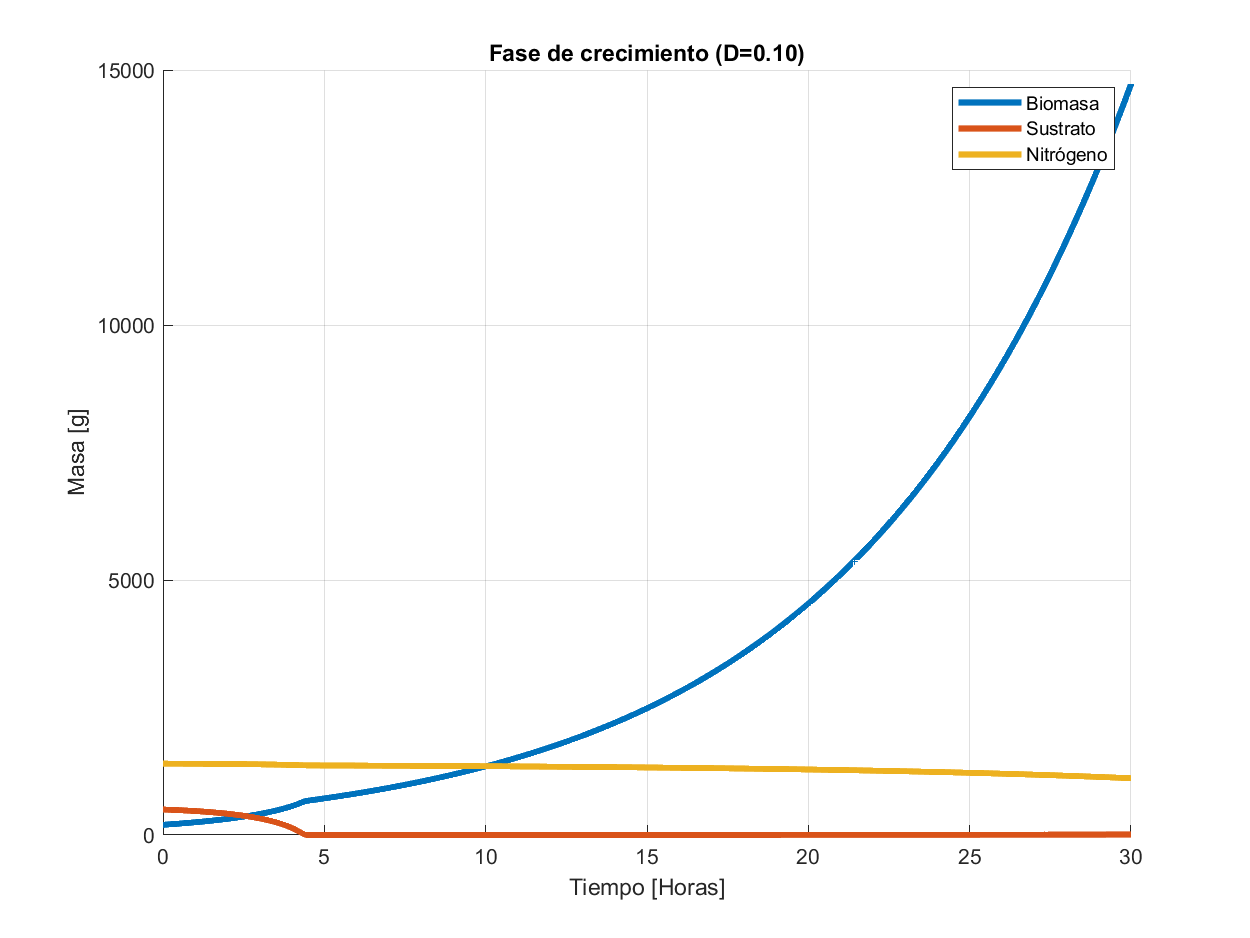
\includegraphics[width=0.43\textwidth]{./Images_tp1/D1_growth_complete_2.png}
  \caption{Fase de crecimiento con alimentación constante}
\end{figure}
\begin{figure}[H]
  \centering
  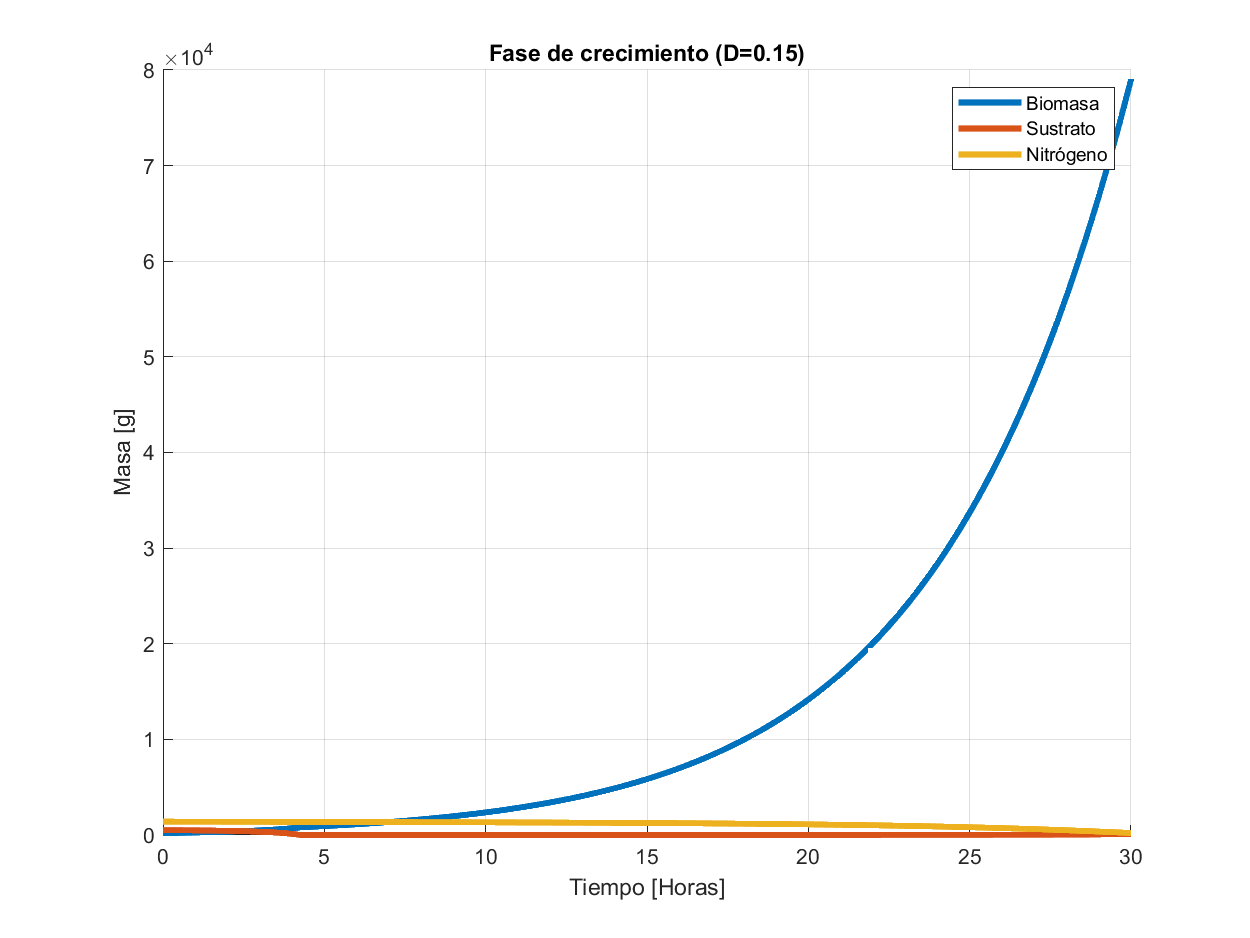
\includegraphics[width=0.43\textwidth]{./Images_tp1/D1_growth_complete_3.png}
  \caption{Fase de crecimiento con alimentación constante}
\end{figure}
\begin{figure}[H]
  \centering
  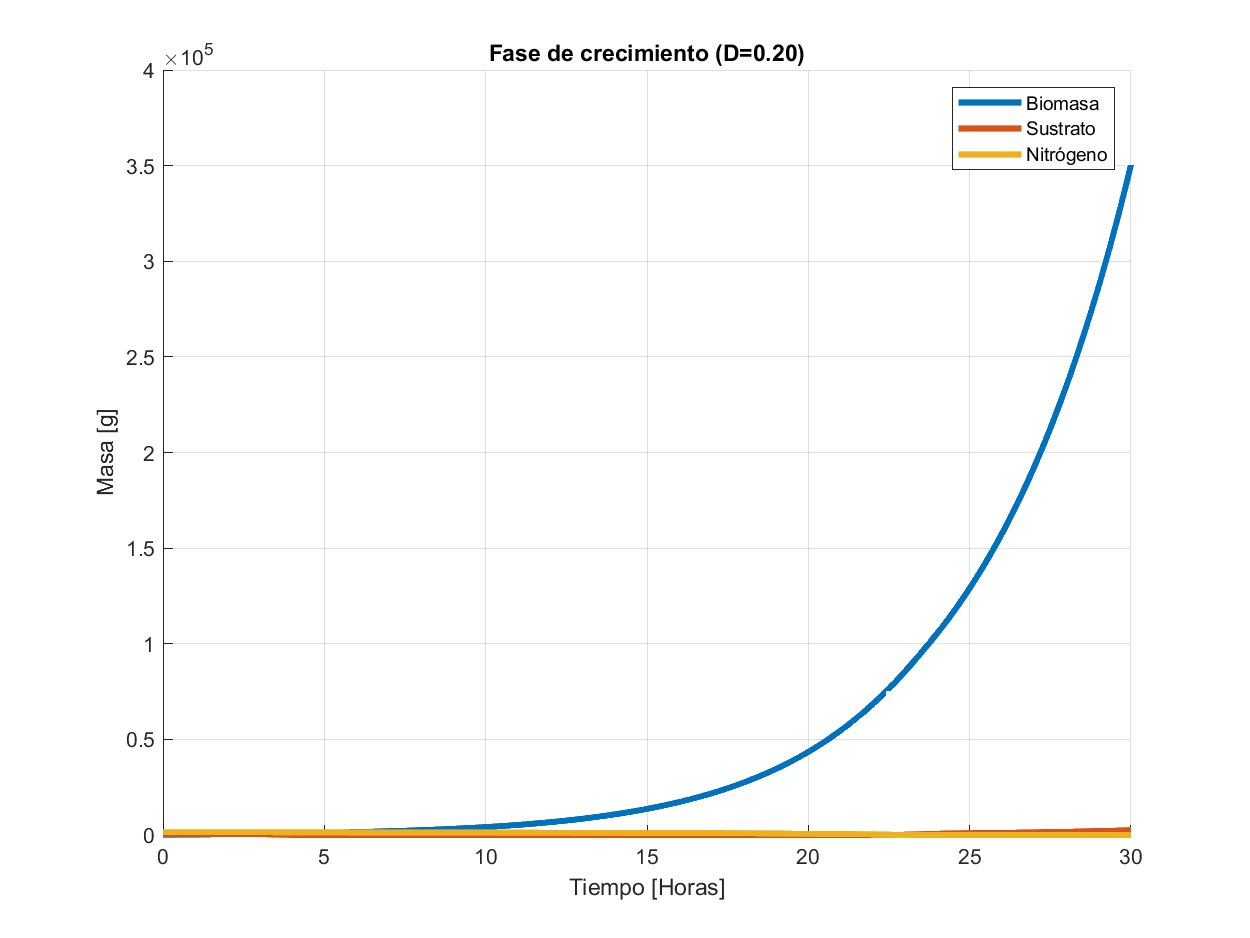
\includegraphics[width=0.43\textwidth]{./Images_tp1/D1_growth_complete_4.png}
  \caption{Fase de crecimiento con alimentación constante}
\end{figure}

Como se puede observar en los gráficos, si se alimenta con poco no se llega a alimentar la biomasa, pero si se alimenta con demasiado sustrato entonces el mismo comienza a acumularse. En las siguientes simulaciones se toma un valor de dilución $D=0.1$, ya que es equilibrado con respecto a lo mencionado anteriormente.

\begin{figure}[H]
  \centering
  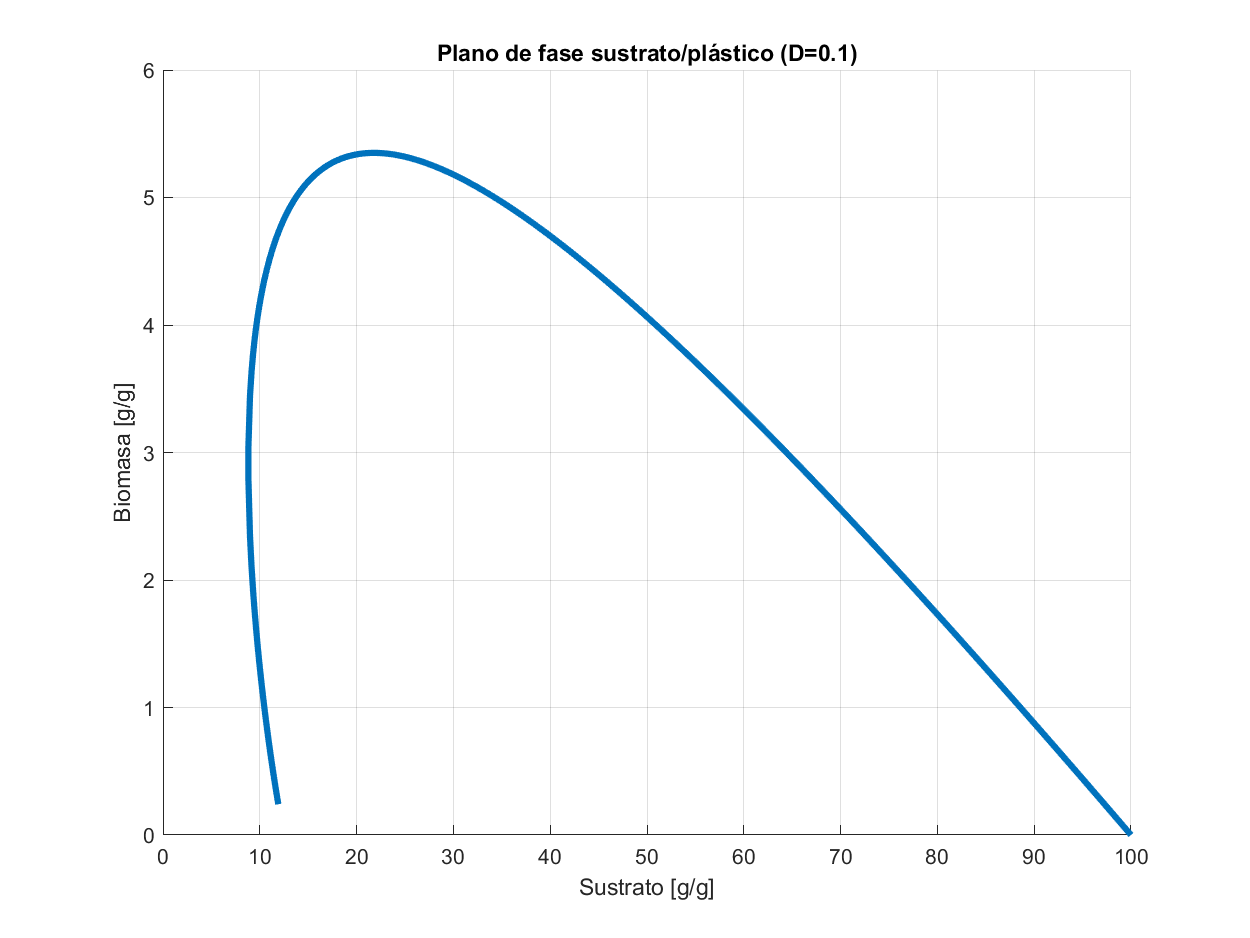
\includegraphics[width=0.43\textwidth]{./Images_tp1/D1_plano_fase.png}
  \caption{Plano de fase en la fase de crecimiento de biomasa}
\end{figure}

\section{Con alimentación de sustrato exponencial}

Se emplea el siguiente modelo para la alimentación exponencial:

\begin{equation*}
D = \frac{K_{s}\mu_{r}x_{0}e^{t*\mu_{r}}}{S_{in}-S_{r}}
\end{equation*}


\end{document}